% RWC 2027 contributed talk proposal: zkEMV.
% Limit: three pages plus references (https://rwc.iacr.org/2027/contributed.php).
% Body and speaker bio must end on page 3; references may continue onto page 4.
\documentclass[10pt,a4paper]{article}

\usepackage[T1]{fontenc}
\usepackage{newtxtext,newtxmath}
\usepackage[margin=2cm]{geometry}
\usepackage{microtype}
\usepackage{booktabs}
\usepackage{enumitem}
\usepackage{tikz}
\usetikzlibrary{arrows.meta,positioning}
\usepackage[hidelinks]{hyperref}

\setlist{nosep}

\title{zkEMV: Private Credentials from EMV Offline Data Authentication}
\author{Anjan Roy (presenting author)\\Radboud University and Avail\\\texttt{anjan.roy@ru.nl}}
\date{}

\begin{document}
\maketitle

\begin{abstract}
EMVCo reports over 15.6 billion EMV chip cards are in use.
Each chip-card authenticates itself to readers, often the in-store payment terminals, through an \emph{offline data authentication} (ODA) step.
ODA requires the card chip to sign a fresh challenge from the reader, with a key that an RSA certificate chain ties to the certification authority (CA).
We show that ODA already gives us a privacy-preserving credential using zero-knowledge cryptography, without any change to card chip, issuers or payment networks.
In \emph{zkEMV}, the user taps their contactless card on their own NFC-capable device, which participates in ODA.
The captured transcript of communication over NFC is used for locally proving that a genuine EMV card signed a challenge nonce presented by the verifier, and that its issuer and card certificates are not expired.
The verifier receives a zero-knowledge proof (ZKP) which it can instantly verify against root of trust CA public key without ever needing to see the card number, expiry dates or none of its certificates.
The ZKP carries a verifier-scoped 32-byte nullifier hash that is linked to the card's ICC public key, resisting Sybil attack vector.
On verifier's request the client can selectively disclose some attributes derivable from the card's bank identification number (BIN), i.e., first 6 to 8 digits of card number, such as, card issuing country, bank or nature of card funding.
Proving runs entirely on user-owned device: when a Samsung Galaxy S25 Ultra is running on battery power, it takes 700ms for a Visa card and 800ms for a Mastercard, to prove ODA in zero-knowledge using Provekit, which implements a Spartan-based sumcheck protocol with WHIR polynomial commitment scheme.
Verification of zkEMV proof takes under 100ms and proof size ranges in 620-640KiB.
The talk presents the zkEMV protocol, with optimizations for sub-second latency client-side proving of ODA, followed by demonstrating practical use cases it opens doors to, which preserves user privacy and reduces merchant liability when handling personally identifiable informations (PIIs).
\end{abstract}

\section{Motivation}
Services that give new accounts something of value, such as free AI and compute credits, privacy-focused email, code hosting or testnet faucets, fight multi-account abuse by collecting identity.
Stripe reports that 7.4\% of sign-ups at AI companies are implicated in suspected multi-account abuse~\cite{stripe-abuse}.
The usual defences are phone numbers, ID uploads, or a card on file that the processor fingerprints for ``one trial per card''.
Card networks and processors now also offer tap-to-verify products~\cite{visa-tap,mc-tap-to-verify,stripe-tap-to-add}.
In every case the relying party or its processor learns the card or the person, and keeps a database that can be breached.

Yet each of the 15.6 billion EMV chip cards in use~\cite{emvco-stats} already carries a better primitive.
During offline data authentication (ODA)~\cite{emv-book2}, a contactless card sends the reader a certificate chain and signs the reader's nonce  a key held in its secure element.
The credential is already issued, so nobody needs to enrol.
Privacy Pass and Private Access Tokens~\cite{privacypass,apple-pat} rely on a platform attester, and proof-of-personhood schemes~\cite{borge-pop} rely on enrolment.
Here no issuer, network or attester takes part.
The certificates, however, embed the PAN, so verifying the chain on a server would hand the server the PAN.
Zero knowledge keeps the PAN off the server.
Zero-knowledge proofs over existing credentials, such as mdoc  ECDSA~\cite{frigo-shelat}, JWT and mDL~\cite{crescent}, OpenID Connect~\cite{zklogin} and legacy signatures~\cite{legacy-sigs}, need enrolment  a government or an identity provider.
zkEMV instead uses a chip that many people already carry, and that chip signs \emph{this verifier's} fresh nonce under a legacy RSA chain.
To our knowledge, no earlier work proves EMV offline data authentication in zero knowledge.

\section{The protocol}
\begin{figure}[t]
\centering
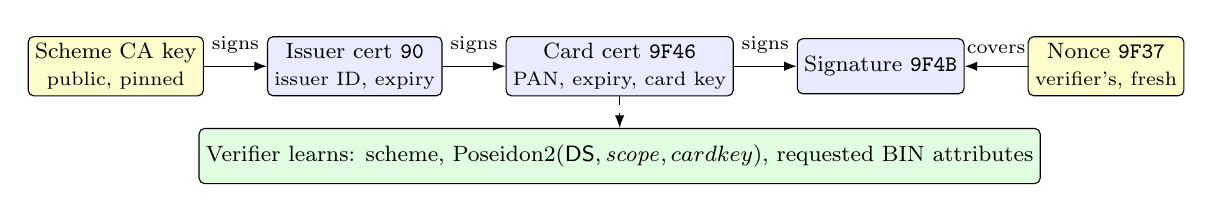
\begin{tikzpicture}[font=\footnotesize, node distance=8mm,
  box/.style={draw, rounded corners=2pt, inner sep=2.5pt, align=center, minimum height=7mm},
  arr/.style={-{Latex[length=1.6mm]}}]
  \node[box, fill=yellow!20] (ca) {Scheme CA key\\\scriptsize public, pinned};
  \node[box, fill=blue!8, right=of ca] (iss) {Issuer cert \texttt{90}\\\scriptsize issuer ID, expiry};
  \node[box, fill=blue!8, right=of iss] (icc) {Card cert \texttt{9F46}\\\scriptsize PAN, expiry, card key};
  \node[box, fill=blue!8, right=of icc] (sdad) {Signature \texttt{9F4B}};
  \node[box, fill=yellow!20, right=of sdad] (nonce) {Nonce \texttt{9F37}\\\scriptsize verifier's, fresh};
  \draw[arr] (ca) -- node[above=1pt]{\scriptsize signs} (iss);
  \draw[arr] (iss) -- node[above=1pt]{\scriptsize signs} (icc);
  \draw[arr] (icc) -- node[above=1pt]{\scriptsize signs} (sdad);
  \draw[arr] (nonce) -- node[above=1pt]{\scriptsize covers} (sdad);
  \node[box, fill=green!12, below=4mm of icc] (out) {Verifier learns: scheme, $\mathrm{Poseidon2}(\textsf{DS}, \mathit{scope}, \text{card key})$, requested BIN attributes};
  \draw[arr, dashed] (icc.south) -- (out.north);
\end{tikzpicture}
\caption{The chain proved in zero knowledge.
Yellow: public inputs.
Blue: private, read from the card.
Green: output.
Each ``signs'' arrow is RSA  $e=3$ and ISO/IEC 9796-2 message recovery over SHA-1.}
\label{fig:chain}
\end{figure}

\paragraph{Flow.}
(1)~The verifier issues a challenge.
It holds a random 4-byte nonce, the current month, a \emph{scope} and an optional request for card attributes.
Visa cards also sign an amount and a currency, which the verifier sets to zero.
(2)~The phone fetches the challenge over TLS and derives the scope itself from the origin it authenticated.
(3)~The user taps.
Mastercard cards sign the nonce in reply to INTERNAL AUTHENTICATE (DDA)~\cite{emv-c2}.
Visa cards sign it in their reply to GET PROCESSING OPTIONS (fDDA)~\cite{emv-c3}.
Cards that support only combined authentication (CDA) are not handled yet.
(4)~The phone proves the statement below, then sends the proof.
(5)~The verifier checks that the proof's public inputs equal its challenge and a CA key it pins, then verifies the proof.
A type-state API keeps the nonce out of the caller's hands and makes each challenge single-use.
This matters because the ProveKit verifier checks a proof only against the public inputs the proof itself carries.

\paragraph{Statement.}
The public inputs are the scheme CA modulus, the nonce, the month, the scope, and the attribute request  its BIN-table root (below).
The witness is what the card sent.
For each of the three signatures (Fig.~\ref{fig:chain}), the circuit:
\begin{itemize}
\item recovers $m = s^3 \bmod n$ and enforces $m<n$, so the bytes it reads are canonical;
\item checks every fixed field of the 9796-2 encoding~\cite{iso9796-2}: header, trailer, format, algorithm indicators, key length and exponent;
\item recomputes the embedded SHA-1 over the recovered body plus the key remainder and signed static data, or plus the terminal data that contains the nonce;
\item rebuilds the next public key from the recovered bytes, checking its padding.
\end{itemize}
Across the chain, the issuer identifier must match the PAN prefix and both certificates must be unexpired.
Every predicate is computed from certificate-recovered bytes, never from the unsigned tags the card also sends, a recurring lesson of the EMV break-and-fix literature~\cite{basin-emv}.

\textbf{Output.} The circuit outputs a nullifier $\mathrm{Poseidon2}(\textsf{DS}, \mathit{scope}, \text{card key})$~\cite{poseidon2}, computed from the card's certified public key.
It is never computed from the PAN, which can be brute-forced within a BIN.
The scope makes the nullifier one of three kinds:
\begin{itemize}
\item \emph{Per verifier}, for example for a free trial.
The phone derives the scope from the authenticated origin, so a site that relays another verifier's challenge obtains only its own nullifier.
\item \emph{Per event}, for example for a poll.
Rounds are unlinkable.
\item \emph{Unlinkable}.
The phone draws a random scope, and the verifier learns only that a genuine card is present.
\end{itemize}
On request, the circuit also reveals coarse attributes: issuer country, credit, debit or prepaid, brand, and consumer or commercial.
It does this  a range proof of the first 12 PAN digits, taken from the issuer-signed card certificate, against a Poseidon2 Merkle root of a BIN table the verifier commits to.
For example, a verifier can turn away cheap prepaid cards without learning the bank.

\section{Use cases}
A card tap fits where a fake account costs the service money, but less than another physical card, and where no payment takes place.
\begin{itemize}
\item \textbf{Free tiers and trials} (per verifier).
AI and compute credits, privacy-focused email and code hosting can grant one free tier per card, storing nothing but the nullifier.
\item \textbf{Bans that stick} (per verifier).
A ban attaches to the nullifier, so coming back takes a new physical card, not a new email address.
\item \textbf{One vote per card} (per event).
Polls, petitions and funding rounds count each card once, and rounds stay unlinkable.
When the verifier is public, as for testnet faucets or quadratic funding~\cite{quadratic-funding}, zero knowledge is required, not optional.
\item \textbf{Confirming a risky action} (per verifier).
Before a payout-address change or an account deletion, the service checks that the tap returns the enrolled card's nullifier.
A stolen card still passes, so the tap complements a password rather than replacing it.
\item \textbf{Bot friction} (unlinkable).
The service learns only that a genuine card is present.
\item \textbf{Coarse gates} (BIN attributes).
A verifier can refuse prepaid cards or restrict access by issuer country.
\end{itemize}
Anti-abuse aggregators such as Human Passport~\cite{human-passport} could accept a zkEMV proof as one signal among several.

\section{Client-side proving}
The prover runs on the user's own phone, so card data never leaves the device that read it.
The circuits are written in Noir~\cite{noir} and proved  ProveKit~\cite{provekit}, which World uses for World~ID~\cite{world-provekit}.
ProveKit pairs a Spartan-style sumcheck~\cite{spartan}  the WHIR polynomial commitment~\cite{whir} over BN254,  no trusted setup.
ProveKit gets zero knowledge from a small masking polynomial and a few blinding polynomials~\cite{world-provekit}.
Each card profile has its own circuit, which fixes the key widths at compile time.
The circuit's shape therefore does not depend on the card's data, and neither does the prove time.

\begin{table}[ht]
\centering
\begin{tabular}{@{}lcc@{}}
\toprule
& Visa fDDA & Mastercard DDA \\
\midrule
Key widths (CA / issuer / card), bits & 1984 / 1408 / 1024 & 1984 / 1920 / 1152 \\
R1CS constraints (whole statement) & 64,702 & 93,054 \\
Prove on the phone & 660\,ms & 823\,ms \\
Verify & 85\,ms & 91\,ms \\
Proof size & 616.6\,KiB & 636.2\,KiB \\
\bottomrule
\end{tabular}
\caption{Proving and verifying on a Galaxy S25 Ultra (Snapdragon 8 Elite, Android 16), on battery.}
\end{table}

This is slower than the few hundred milliseconds that Frigo and shelat report for mdoc proofs on a phone~\cite{frigo-shelat}.
Our statement covers three RSA recoveries and about 1\,KiB of SHA-1 input.
The lessons carry over to other legacy-signature circuits:
\begin{itemize}
\item \textbf{SHA-1 dominates, not RSA.} With $e=3$, a 1984-bit 9796-2 recovery costs about 3.5k constraints.
That is two products, each checked as a polynomial identity over 120-bit limbs,  limb and carry bounds that make it hold over the integers.
SHA-1 makes up about three-quarters of each circuit, so its layout decides the cost.
It is built around lookup tables, where a single read both range-checks a chunk and spreads it for bitwise operations,  one witness hint per block.
A block costs 4.6k constraints, less than half the 10.6k of a general-purpose Noir SHA-1.
\item \textbf{Count padded witnesses, not constraints.} ProveKit sizes its commitments by the next power of two of the witness count.
Prove time therefore changes only when the witness count crosses a power of two, and saving constraints below that boundary does not shorten proving.
\item \textbf{Poseidon2, not Keccak, for hashing in the circuit.} The nullifier and the BIN Merkle tree both need a hash inside the circuit.
ProveKit does not support Keccak natively, and Keccak written in plain Noir costs 180k constraints per permutation.
ProveKit does support Poseidon2 natively, at 268 constraints per permutation, so we use Poseidon2.
\end{itemize}

\section{Limitations}
A proof is about a card, not a person.
A tap sets a cost floor of one physical chip card per account per verifier.
Virtual card numbers and phone wallets cannot be tapped, and the BIN attributes let a verifier refuse cheap prepaid cards.
A proof also shows only that a genuine card answered somewhere.
NFC relay is commodity crime~\cite{eset-ngate,threatfabric-ghosttap}, but the per-verifier nullifier still caps a rented card at one account per verifier.
In the \emph{unlinkable} scope, a proof that is not bound to the verifier's origin would let a malicious site launder its users' taps through another verifier's presence check.
Binding an origin hash in every scope stops this.

Privacy holds against the verifier, not against everyone.
The nullifier is unkeyed: the issuer, the network, and every terminal or skimmer that has read a card can compute it in any scope, including in unlinkable proofs, whose random scope is public.
zkEMV therefore reduces downstream copies of card data, but hides nothing from the payment rails.
The anonymity set is also smaller than all cards.
A proof reveals its circuit and therefore the card's key-width profile, which today is one per scheme.
Requested BIN attributes narrow it further: in our table~\cite{binlist-data}, 0.25\% of ranges are unique on all four attributes.
A verifier-chosen BIN table  fine ranges could leak the PAN prefix, so the phone must pin the roots it accepts.

zkEMV inherits offline EMV's security: SHA-1~\cite{sha1-shambles}, 1984-bit RSA, the ISO/IEC 9796-2 forgery literature~\cite{cntw}, and a 4-byte nonce, so an attacker who harvested $k$ signatures succeeds  probability $k\cdot 2^{-32}$ per challenge.
Revocation is not checked.
No official public distribution of CA keys exists.
Ours come from community lists~\cite{eftlab-ca-keys} and are authenticated only because real certificates verify under them.
ProveKit was audited by Least Authority~\cite{world-provekit}, but our circuits have not been audited.

The phone app sees all card data, so users must trust an open-source app.
On Visa cards the fDDA read also makes the chip compute a transaction cryptogram, although no payment is made.
The cryptogram must never leave the phone, because it is a pre-play primitive~\cite{chip-and-skim}.
The read also advances the card's transaction counter, which the issuer sees.
iOS restricts reading payment cards~\cite{apple-nfc-payment}, so the system is Android-first.
Finally, EMV's ECC kernel, C-8~\cite{emv-c8}, adds blinded key agreement and may not leave a signature a phone can prove.
Our ask to EMVCo and the networks is to keep a transferable, privacy-preserving attestation in next-generation cards.

\section{Why RWC}
The talk brings a new credential class to RWC: one held by billions of people,  a live hardware challenge.
It is timely because the non-private version of card-tap verification is shipping now.
Attendees will see a working design that is honest about its limits, and techniques for proving legacy RSA, 9796-2 and SHA-1 in a hash-based prover on a phone, which carry over to other legacy credentials.
The talk also raises open questions for EMVCo, wallet vendors and regulators: next-generation card protocols, scheme rules on non-payment reads, and whether the nullifier counts as personal data.

zkEMV is open source under MIT or Apache-2.0~\cite{zkemv-repo}.
It comprises Noir circuits for Visa fDDA and Mastercard DDA, a Rust prover and verifier crate that handles challenges and CA keys, and benchmarks that prove and verify on an Android phone.
The card layouts were taken from captures of real Visa and Mastercard cards, whose chains verify natively under the production CA keys.
The circuits are tested and benchmarked on synthetic taps  the same layouts.
The talk will include a live demo of an Android app that reads a card over NFC and proves on the device.

\section*{Speaker}
\textbf{Anjan Roy} is a PhD candidate in applied cryptography at Radboud University, supervised by Prof. Joan Daemen and Dr. Gilles Van Assche, and leads development of a private payments system based on zero-knowledge proofs at Avail.
Anjan was previously a senior cryptography engineer at the Technology Innovation Institute in Abu Dhabi, building a side-channel-resistant symmetric and post-quantum library, and a blockchain engineer at Polygon Labs, working on a STARK-based zkVM.
Anjan also maintains widely used open-source implementations of post-quantum and symmetric primitives.
Recent talks: RWPQC~2026 (affiliated  RWC~2026, Taipei), the Cedarcrypt~2026 summer school, and GelreCrypt~2025.
Slides: \url{https://itzmeanjan.in/pages/talks.html}.

{\footnotesize
\bibliographystyle{plainurl}
\bibliography{refs}
}
\end{document}
